\chapter{Learning Vector Quantization Neural Network}
\label{chapter:lvq}
\section{簡介}

%%圖\ref{fig:LvqNetwork}爲LVQ的網路架構圖。SOM是一個分群的演算法,如果將它的概念轉成監督式學習,就是LVQ演算法的由來。這個演算法可用於分類的應用,且具有簡單的架構。

學習向量量化(Learning Vector Quantization,簡稱爲LVQ),可以將其視爲是一種人工神經網路的特例。
圖\ref{fig:LvqNetwork}爲LVQ的網路架構圖。
從圖中可以發現這個網路僅具有輸入與輸出兩層,所以是一個結構相當簡單的神經網路,並且是一個具有監督式學習的分類演算法。
此外,在這個演算法中,採取了非監督式學習的機制,應用於監督式學習的問題上。

\begin{figure}[h]
	\centering
	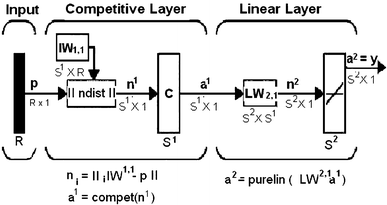
\includegraphics[width=10cm]{./pic/lvq_struct.png}
	\caption{LVQ網路架構圖}
	\begin{minipage}{.7\linewidth}
		\footnotesize
		\emph{圖片來源:}取自Seafloor sediment classification from single beam echo sounder data using LVQ network
	\end{minipage}
	\label{fig:LvqNetwork}
\end{figure}
\label{sec:background}


\section{Vector Quantization}
在理解LVQ演算法前,我們先來看看Vector Quatization。這個算法的目的主要是將原資料分割k個域區,並在這些分割的區域中,找出一個最能代表整個群組的向量,作為這個區域中的代表點。
這些代表點的集合我們稱爲codebook。
此外這個算法所做的事情有點類似將資料進行分群。
LVQ就是基於這個演算法的概念進行,透過監督式學習,不斷的更新代表的位置,進而找出最佳的codebook。


從圖\ref{fig:DataAfterVq},可以看到原資料被分割成3個區域,以及3個紅色方點,而紅色方點就是整個分割區域中的代表點,也是LVQ中的weight vetcor。


\begin{figure}[h]
	\begin{center}
		\begin{tabular}{ccccccccccccc}
			\subfigure[原資料集分佈]{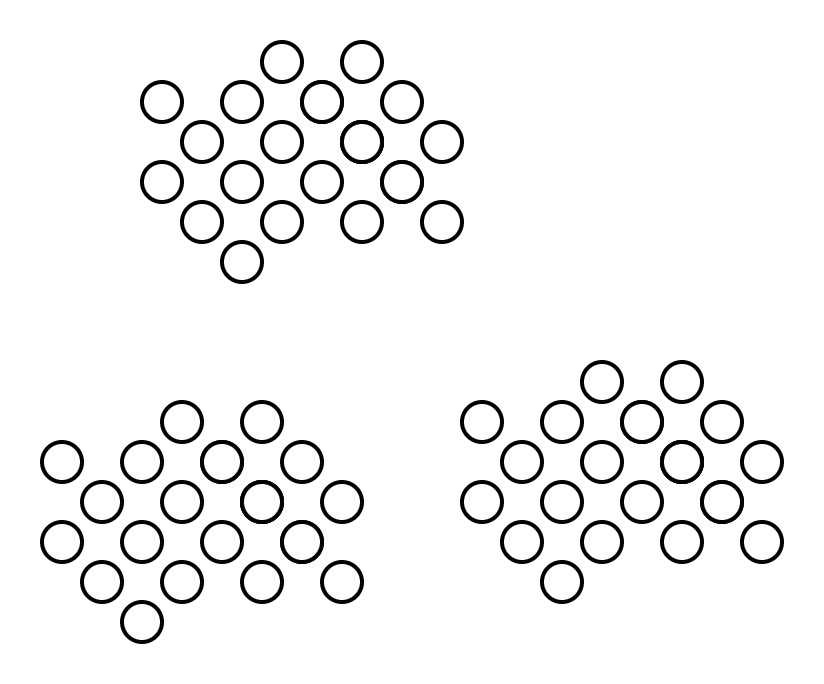
\includegraphics[height=4cm]{./pic/oA5nFv7C.png}\label{fig:ori_data} } \par &
			\subfigure[經過向量量化的原資料]{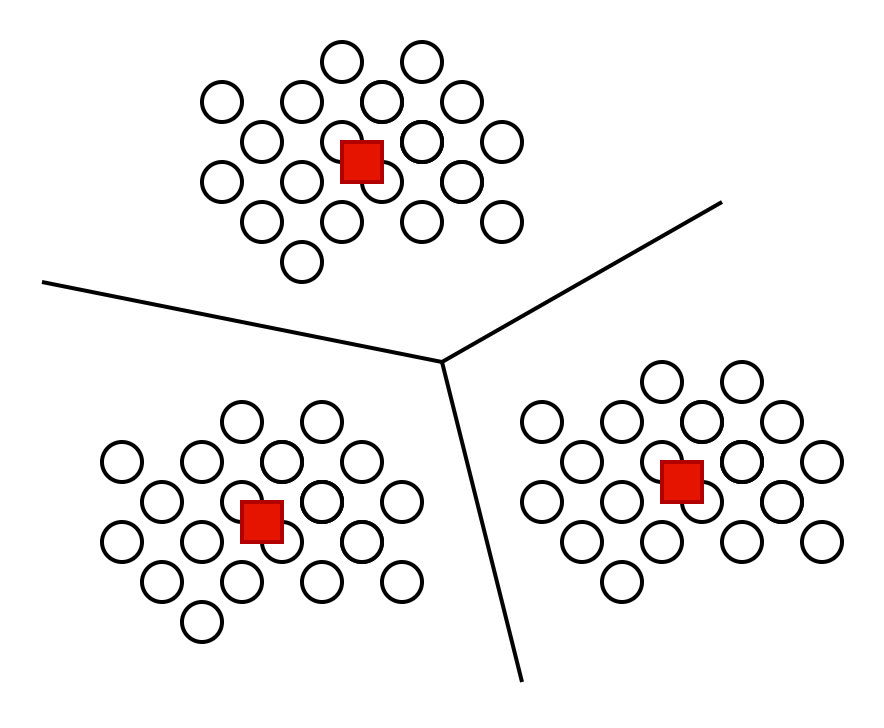
\includegraphics[height=4cm]{./pic/aLVdIIWU.png}\label{fig:DataAfterVq} } \par \\
		\end{tabular}
		\caption{向量量化的示意圖}
		\label{fig:VectorQuantization}
	\end{center}
\end{figure}



%%- 權重向量爲,$$\mathbf{w_{j}} = (w_{1j},w_{2j},w_{3j},....,w_{nj})$$
%%- 距離的計算採用,尤拉距離公式 $$D(j)=||\mathbf{x}-\mathbf{w_j}||_2 = \sqrt{(x_1-w_{1j})^2+(x_2-w_{2j})^2+...+(x_n-w_{nj})^2} $$
%%- $$C_j$$ 為網路層的輸出類別。
%%- $$T$$ 為每筆資料所對應的實際類別。
%%- $$\alpha$$爲學習率


\section{演算法參數定義與流程}

%%在這個演算法中只有Input Layer與Output Layer

\subsection{參數定義}

\begin{itemize}
	\item
	      輸入向量,\(\mathbf{x} = (x_1,x_2,x_3,....,x_R)\),爲資料集中的其中一筆資料,輸入向量的數量 \(d\) 爲資料的特徵數量。


	      %
	\item
	      競爭層權重,\(\mathbf{W^1} = (\mathbf{w_1,w_2,...,w_j,...w_R})^T\),爲一個 \(S^1 \times R \)的矩陣,也就是剛剛介紹Vector Quantization所提到的codebook,這邊的 \(n\)爲輸出的類別數量。
	      %
	\item
		權重向量,\(\mathbf{w_{j}} = (w_{1j},w_{2j},w_{3j},....,w_{dj})^T\),代表每個區域的代表點。

	      %
	\item
	      \(D(j)\)爲每筆資料與代表點的距離。
	      $$D(j)=||\mathbf{x}-\mathbf{w_j}||_2 = \sqrt{(x_1-w_{1j})^2+(x_2-w_{2j})^2+...+(x_n-w_{nj})^2} $$


	\item
	      %\(C_j\) 為網路層的輸出類別。
		\(\mathbf{C}\) 為競爭層的輸出向量。

	\item
	      輸出層權重,\(\mathbf{W^2} \)為一個 \(S^2 \times S^1\)的矩陣。

	\item
		\(\mathbf{y}\) 為網路的輸出向量。

	\item
	      \(\alpha\) 爲學習率
	\item
		此外,這裡為了方便說明,將 \(\mathbf{W^2}\) 設定為一個 \(S^1 \times S^1\) 的單位矩陣,也因此競爭層的輸出為網路層的輸出 \(\mathbf{C} = \mathbf{y}\)。

\end{itemize}


\subsection{流程}

首先會先初始化 \(\mathbf{W^1},\alpha\),接著將所有的訓練資料集中的每一筆資料,找出與每筆資料最近權重向量,並接著判斷 \(\mathbf{y}\) 的結果是否符合這筆資料的類別,如果相同就使得這個權重向量靠近這筆資料點且更新學習率,反之,如果不同則遠離。接著不斷重複以上步驟,直到訓練次數或是學習率達到設定的標準,則停止模型訓練。下圖爲演算法的流程圖\ref{fig:AlogrithmWorkflow}。

\newpage

\usetikzlibrary{positioning, shapes.geometric}

\tikzset{every picture/.style={line width=1.75pt}}


\begin{figure}
	\centering
	
	\resizebox{300pt}{400pt}{
		\begin{tikzpicture}[scale=1]
			\node[draw, rounded corners,align=center ]                        (start)   {初始化參數 \(\mathbf{W},\alpha\) };
			\node[draw,diamond, below=20pt of start,align = center]                        (step 2)  {訓練 \(\mathbf{x}\) 中的\\每一筆資料};
			\node[draw,  aspect=2, below=20pt of step 2]     (step 3)  {找出 \(min\{D(1),D(2),...,D(j),..D(d)\}\) };
			\node[draw, diamond,below=20pt of step 3]                   (compare)  {比對 \(y\)與 \(T\)  };
			\node[draw, below =30pt of compare,align = center]                         (same)  {\(\mathbf{w_j(new)} = \mathbf{w_j(old)} + \alpha(\mathbf{x} - \mathbf{w_j(old)})\)  };
			\node[draw, below right=55pt and 80pt of compare]                         (different)  {\(\mathbf{w_j(new)} = \mathbf{w_j(old)} - \alpha(\mathbf{x} - \mathbf{w_j(old)})\)};
			\node[draw, rounded corners, below=20pt of same]  (learning_rate)     {更新學習率 \(\alpha\) };
			\node[draw,diamond, below=20pt of learning_rate,align = center]                         (end_detect)  {判斷是否\\達到結束條件};
			\node[draw, rounded corners, below=20pt of end_detect]  (end)     {End};

			\draw[->] (start)  --coordinate(le) (step 2);
			\draw[->] (step 2) --node[left]{Yes} (step 3);
			\draw[->] (step 2.west) --node[above]{Yes}++(-50pt,0)|-(end_detect.west);
			\draw[->] (step 3) -- (compare);
			\draw[->] (compare) -> node[left]{Yes}(same.north);
			\draw[->] (compare.east) --node[above]{No}(compare.east-|different.north) -> (different.north);
			\draw[->] (same) -- (learning_rate);
			\draw[->] (learning_rate) -> (end_detect);
			\draw[->] (end_detect) -- node[left]{Yes}(end);
			\draw[->] (end_detect.east) --node[above]{No}++(250pt,0pt)|-(le) ;

		\end{tikzpicture}
	}

	\caption{演算法流程圖}
	\label{fig:AlogrithmWorkflow}
\end{figure}



%要被單行註解的文字。

\begin{comment}
要被區塊註解的文字,要被區塊註解的文字,要被區塊註解的文字,
要被區塊註解的文字,要被區塊註解的文字,要被區塊註解的文字,
要被區塊註解的文字,要被區塊註解的文字,要被區塊註解的文字,
要被區塊註解的文字,要被區塊註解的文字,要被區塊註解的文字,
要被區塊註解的文字,要被區塊註解的文字,要被區塊註解的文字,
要被區塊註解的文字,要被區塊註解的文字。
\end{comment}

\section{實例說明}

爲了能夠更簡單理解這個演算法的目的與實際的效果,以下以簡單的實例說明。
表\ref{tab:lvq_table}爲此次實例的資料集,此資料集分別有x跟y兩個特徵,以及兩種類別,並分別以綠色與紅色表示。


\begin{table}[h!]
	\centering
	\caption{資料集}
	\label{tab:lvq_table}
	\begin{tabular}{rrrr}
\toprule
  & x & y & Class  \\
\midrule
 & 1  & 3  & 1     \\
 j 6  & 1  & 2     \\
 & 3  & 4  & 1      \\
 & 8  & 3  & 2     \\
 & 9  & 1  & 2     \\
 & 1  & 6  & 1 	\\     
\bottomrule
\end{tabular}

\end{table}


\begin{figure}[h!]
	\centering
	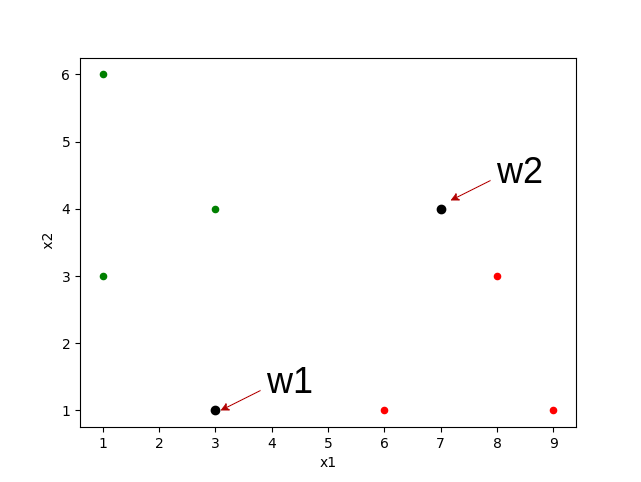
\includegraphics[height=10cm]{./pic/2nSRVeud.png}
	\caption{資料集在座標軸的分佈}
	\label{fig:DatasetInAxis}
\end{figure}

\newpage
\begin{enumerate}
	\item
	      首先先初始化 \(\mathbf{W}\),因爲這次的範例中只有兩個類別,這邊以 \(\mathbf{w_1}=(3,1),\mathbf{w_2}=(7,4)\)作爲初始化的兩個weight vector。並將學習率 \(\alpha\)的初始值設爲0.5,以及iteration設定爲100。
	      圖 \ref{fig:DatasetInAxis}爲此資料集與初始兩個weitght在座標軸的分佈。
	      %
	\item
	      接著計算第一筆資料與兩個weight vector的歐式距離,並比較兩個距離的大小。

	      $$D(1)=||\mathbf{x}-\mathbf{w_1}||_2 = \sqrt{(1-3)^2+(3-1)^2}=\sqrt{8}=2.8284 $$
	      $$D(2)=||\mathbf{x}-\mathbf{w_2}||_2 = \sqrt{(1-7)^2+(3-4)^2}=\sqrt{37}=6.0827 $$
	      $$D(1)<D(2)$$

	      %
	\item
	      由上一步得知 \(D(1)<D(2)\),所以此筆資料的神經網路的輸出結果 \(C_1\) 爲1,又因爲 \(C_1 = T = 1\),所以更新 \(\mathbf{w_1}\)要往 \(x\)的方向前進。此外,也因爲輸出結果與實際類別相同所以還要更新學習率的值。
	      $$\mathbf{w_1}(new) = \mathbf{w_1}(old) + \alpha(\mathbf{x-w_1}(old))= \begin{bmatrix}3\\ 1\end{bmatrix}+0.5(\begin{bmatrix}1\\ 3\end{bmatrix} - \begin{bmatrix}3\\ 1\end{bmatrix})= \begin{bmatrix}2\\ 2\end{bmatrix}  $$
	      $$\alpha(new) = \alpha(old)\times \frac{1}{1+decay*iteration} =0.4950$$

	\item
	      接著換第二筆資料
	      $$D(1)=||\mathbf{x}-\mathbf{w_1}||_2 = \sqrt{(6-2)^2+(1-2)^2}=4.1231 $$
	      $$D(2)=||\mathbf{x}-\mathbf{w_2}||_2 = \sqrt{(6-7)^2+(1-4)^2}=3.1622 $$
	      $$D(2)<D(1)$$
	      $$\mathbf{w_2}(new) = \mathbf{w_2}(old) + \alpha(\mathbf{x-w_2}(old))= \begin{bmatrix} 6.5049 \\ 2.5148 \end{bmatrix}  $$
	      $$\alpha(new) = 0.4901$$




	\item
		依序將所有資料集輸入,並依照以上的步驟,比較各個資料與兩個weight vector之間的距離,接著更新權重與學習率。圖\ref{fig:LvqWeightMove}爲第一次迭代的兩個權重的移動路徑。

\begin{figure}[h!]
	\centering
	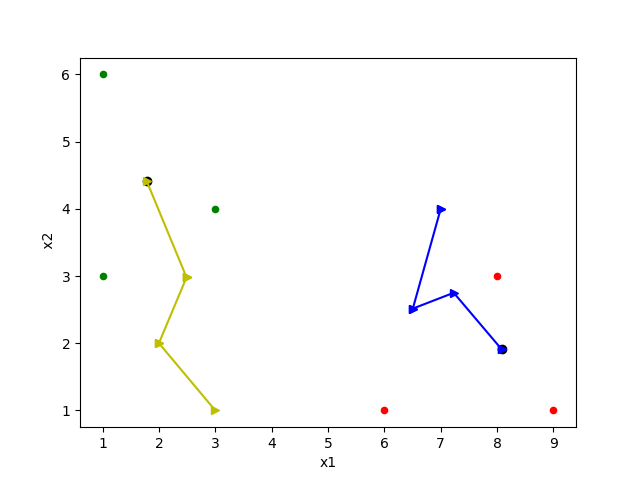
\includegraphics[height=10cm]{pic/lvq_weight_move.png}
	\caption{權重向量第一次迭代的移動路徑}
	\label{fig:LvqWeightMove}
\end{figure}

	      %
	\item 
		不斷重複以上2\char`\~ 5的步驟,直到設定的iteration到100爲止。圖\ref{fig:Lvq100Iteration}爲此資料集經過100次迭代的結果,可以發現權重向量移動的步伐因爲學習率的縮小,移動的越來越小,也因此它的值也漸漸固定不在改變,此外這兩個權重向量分別往兩個類別的群心點靠近。
\begin{figure}[h!]
	\centering
	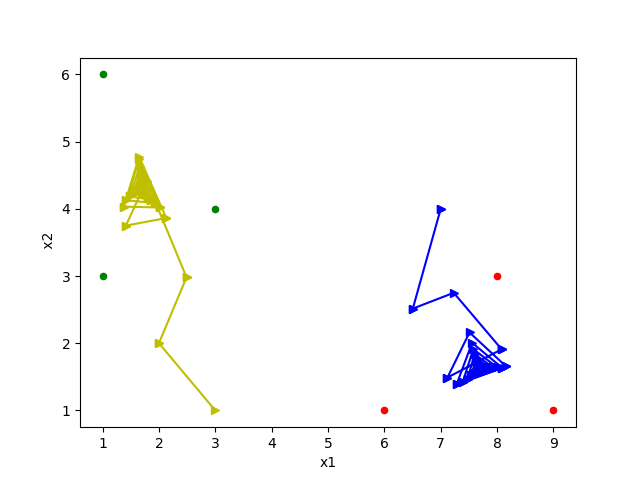
\includegraphics[height=10cm]{pic/lvq_100_iteration.png}
	\caption{經過100次迭代的結果}
	\label{fig:Lvq100Iteration}
\end{figure}

\end{enumerate}


\newpage

\section {結論}
從以上的實例可以發現這個演算法,其實蠻簡單的而且也易於理解,也因爲這個模型的參數較少,所以模型的訓練速度非常的快,以剛剛的資料集,在100次的迭代的情況下,訓練的時間不到15秒即可完成,所以這個演算法在資料集簡單的情況下,是能夠在短時間內訓練出一個不錯的模型。

